\documentclass[12pt]{beamer}
\usepackage{graphicx}
\usepackage{hyperref}
\usepackage{amsmath}
\usepackage{listings}
\usepackage{xcolor}

\usepackage{fontspec}
\usefonttheme[onlymath]{serif}
\newfontfamily\cyrillicfont{CMU Sans Serif}
\newfontfamily\cyrillicfonttt{JetBrains Mono}
\setsansfont{CMU Sans Serif}
\setmonofont{JetBrains Mono}

\usepackage{polyglossia}
\setdefaultlanguage{russian}
\setotherlanguage{english}

\setbeamertemplate{caption}[numbered]
\setbeamertemplate{figure}[numbered]


\usepackage[skip=10pt, labelfont=bf]{caption}
\captionsetup{labelsep=endash}
\addto\captionsrussian{
    \renewcommand{\figurename}{Рисунок}
    \renewcommand{\lstlistingname}{Листинг}
}

\usetheme{Madrid}
\usecolortheme{default}

\title{Классификация изображений с помощью сверточных нейронных сетей}
\subtitle{Курсовая работа}
\author{Нефедов Д.А.}
\institute{МГТУ им. Н.Э. Баумана}
\date{}

\begin{document}
\sloppy

\begin{frame}
    \titlepage
    \begin{center}
        Научный руководитель: Фетисов Д.А.

        {\fontsize{8}{12}\selectfont Москва, 2025 г.}
    \end{center}
\end{frame}

\begin{frame}{Постановка задачи}
    \begin{itemize}
        \item Дано: набор данных с изображениями 10 видов животных: бабочка, паук, собака, слон, овца, кот, корова, белка, лошадь, курица.
        \item Обьем данных: 26 тысяч изображений.
        \item Задача: построение классификатора на основе модели сверточной нейронной сети.
        \item Средства: язык \textbf{Python} и библиотека глубокого обучения \textbf{pytorch}.
    \end{itemize}
\end{frame}

\begin{frame}{Распределение данных}
    \begin{center}
        \textbf{Вывод}: изображения приведены к разрешению $256 \times 256$
    \end{center}
    \begin{figure}[h]
        \centering
        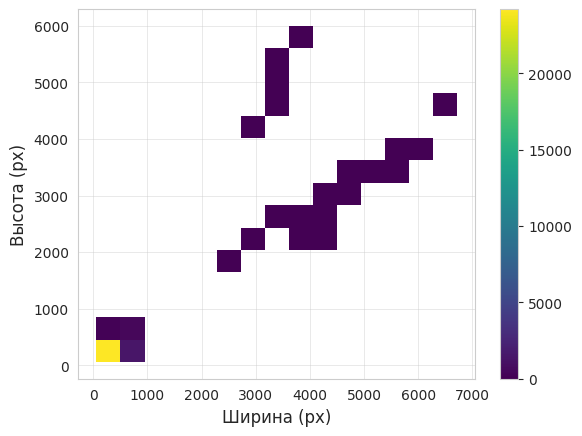
\includegraphics[width=0.6\textwidth]{images/data_dist.png}
        \caption{Распределение данных по разрешениям}
        \label{fig:data_dist}
    \end{figure}
\end{frame}

\begin{frame}{Распределение данных (продолжение)}
    \begin{center}
        \textbf{Вывод}: учитывался баланс классов
    \end{center}
    \begin{figure}[h]
        \centering
        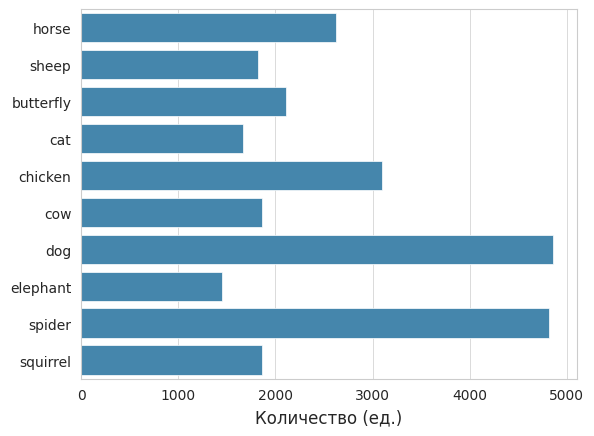
\includegraphics[width=0.6\textwidth]{images/class_dist.png}
        \caption{Распределение данных по классам}
        \label{fig:class_dist}
    \end{figure}
\end{frame}

\begin{frame}{Сверточная нейронная сеть}
    Две интерпретации свертки:
    \begin{itemize}
        \item Классическая: $(X * Y)(t, s) = \sum_{i, j} X_{i,j} \cdot Y_{t - i, s - j}$
        \item Взаимная корреляция: $(X \otimes Y)(t, s) = \sum_{i, j} X_{i, j} \cdot Y_{i + t, j + s}$
    \end{itemize}

    \begin{figure}[h]
        \centering
        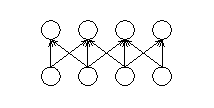
\includegraphics[width=0.6\textwidth]{images/conv.pdf}
        \caption{Сверточный слой}
        \label{fig:conv_layer}
    \end{figure}
\end{frame}

\begin{frame}{Сверточная нейронная сеть (продолжение)}
    \begin{figure}[ht]
        \centering
        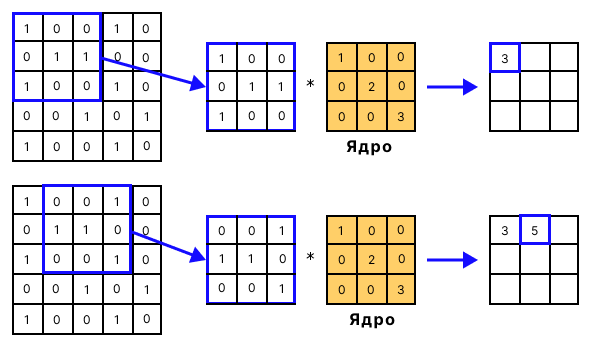
\includegraphics[width=0.8\textwidth]{images/conv_window.png}
        \caption{Визуализация свертки}
        \label{fig:conv}
    \end{figure}
\end{frame}

\begin{frame}{Модель AlexNet}
    \begin{figure}[ht]
        \centering
        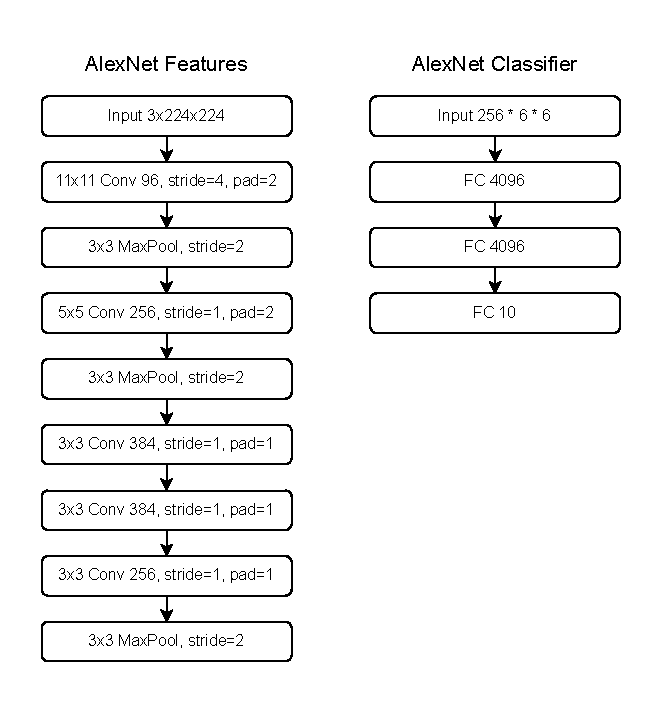
\includegraphics[width=0.5\textwidth]{images/alexnet_model.pdf}
        \caption{Модель AlexNet}
        \label{fig:alexnet}
    \end{figure}
\end{frame}

\begin{frame}{Результаты обучения AlexNet}
    \begin{center}
        \textbf{Вывод}: получена желаемая точность ($>0.85\%$)
    \end{center}
    \begin{figure}[ht]
        \centering
        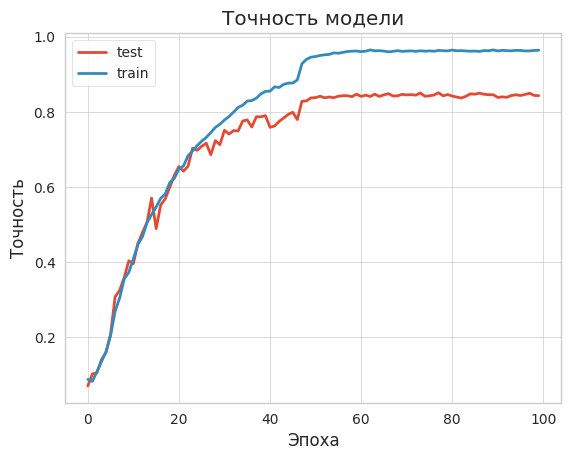
\includegraphics[width=0.6\textwidth]{images/alexnet_lrn_f1.png}
        \caption{График точности AlexNet по эпохам}
        \label{fig:alexnet_f1}
    \end{figure}
\end{frame}

\begin{frame}{Визуализация AlexNet}
    \begin{figure}[ht]
        \centering
        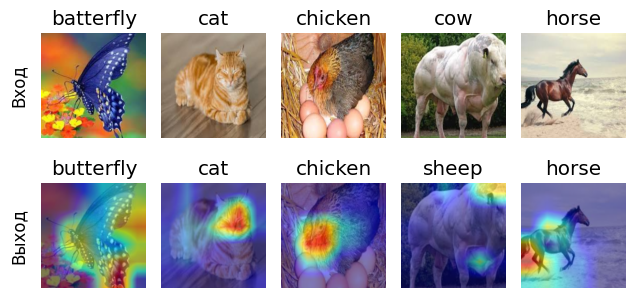
\includegraphics[width=0.9\textwidth]{images/alexnet_out_1.png}
        \caption{Результаты применения Grad-CAM к модели AlexNet}
        \label{fig:alexnet_gradcam_1}
    \end{figure}
\end{frame}

\begin{frame}{Визуализация AlexNet (продолжение)}
    \begin{center}
        \textbf{Вывод}: паук предсказывается по окружению, слабая классификация собаки.
    \end{center}
    \begin{figure}[h]
        \centering
        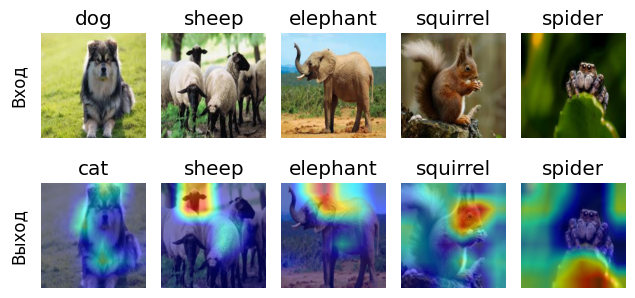
\includegraphics[width=0.8\textwidth]{images/alexnet_out_2.png}
        \caption{\centering Результаты применения Grad-CAM к модели AlexNet (продожение)}
        \label{fig:alexnet_gradcam_2}
    \end{figure}
\end{frame}

\begin{frame}{Модель VGG13}
    \begin{figure}[ht]
        \centering
        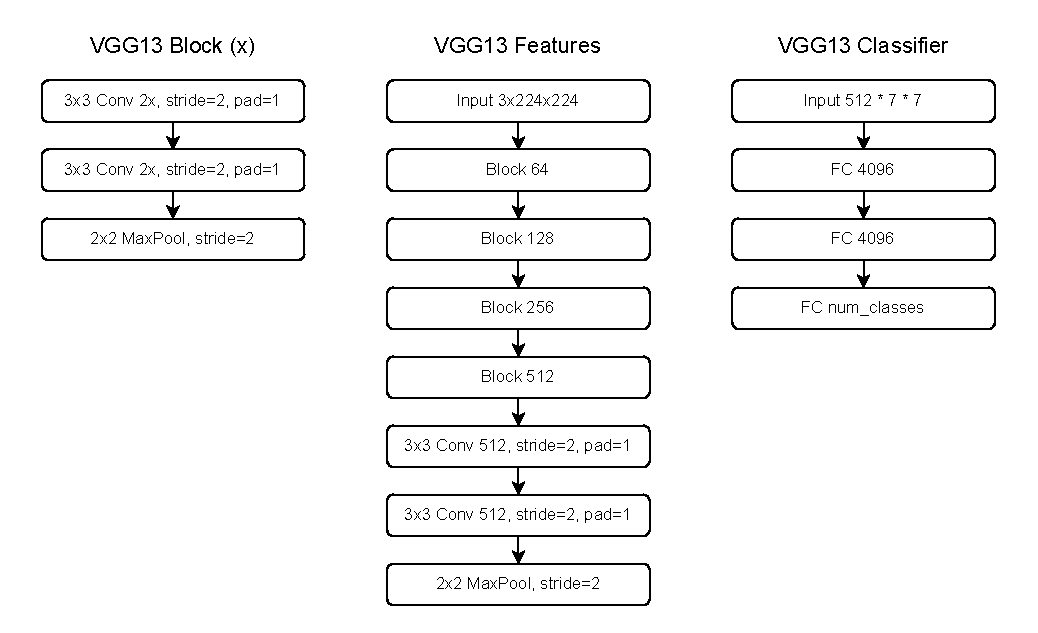
\includegraphics[width=0.8\textwidth]{images/vgg13_model.pdf}
        \caption{Модель VGG13}
        \label{fig:vgg13}
    \end{figure}
\end{frame}

\begin{frame}{Модификация модели VGG13}
    \begin{figure}[ht]
        \centering
        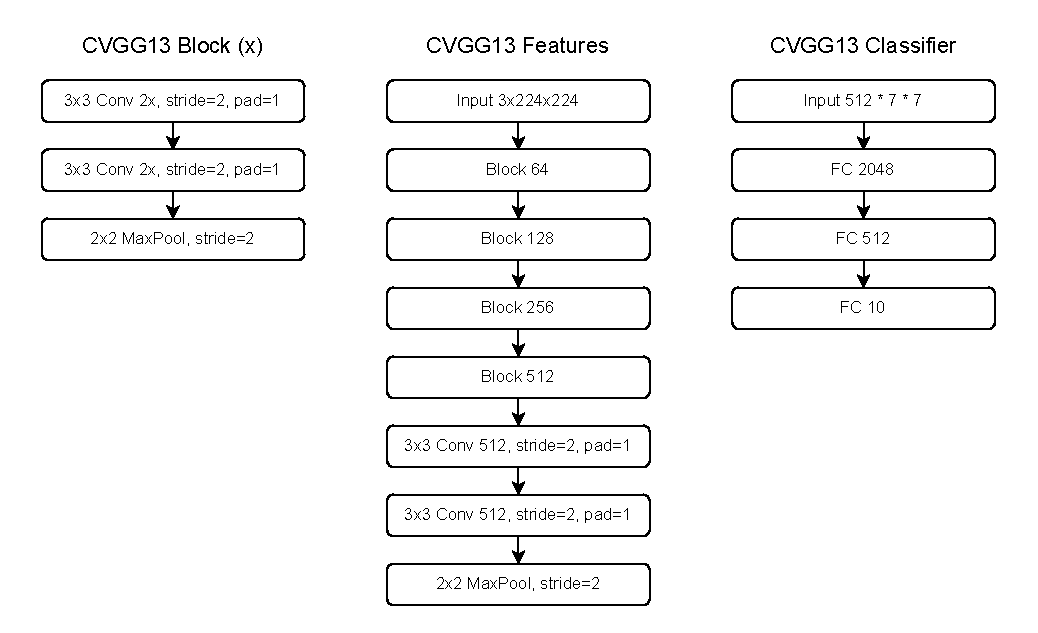
\includegraphics[width=0.8\textwidth]{images/cvgg13_model.pdf}
        \caption{Модификация VGG13}
        \label{fig:cvgg13}
    \end{figure}
\end{frame}

\begin{frame}{Результаты обучения CVGG13}
    \begin{center}
        \textbf{Вывод}: получена лучшая точность ($\approx 0.92\%$)
    \end{center}
    \begin{figure}[ht]
        \centering
        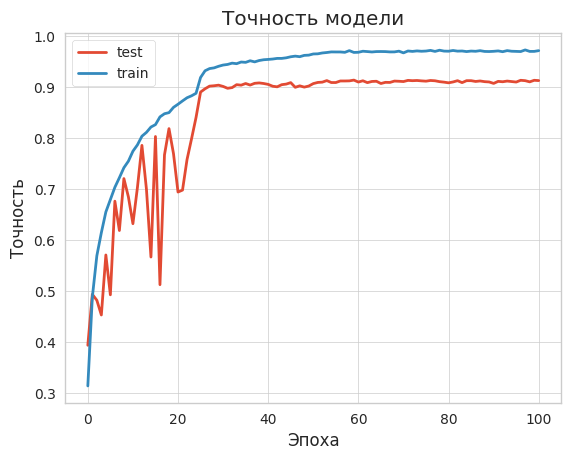
\includegraphics[width=0.6\textwidth]{images/cvgg13_f1.png}
        \caption{График точности CVGG13 по эпохам}
        \label{fig:cvgg13_f1}
    \end{figure}
\end{frame}

\begin{frame}{Визуализация CVGG13}
    \begin{figure}[ht]
        \centering
        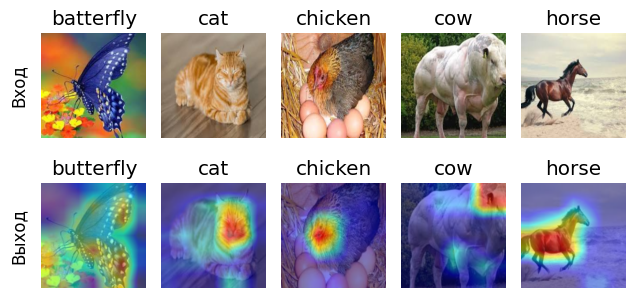
\includegraphics[width=0.9\textwidth]{images/cvgg13_out_1.png}
        \caption{Результаты применения Grad-CAM к модели CVGG13}
        \label{fig:cvgg13_gradcam_1}
    \end{figure}
\end{frame}

\begin{frame}{Визуализация CVGG13 (продолжение)}
    \begin{center}
        \textbf{Вывод}: корректно выделенные признаки, в отличие от AlexNet
    \end{center}
    \begin{figure}[h]
        \centering
        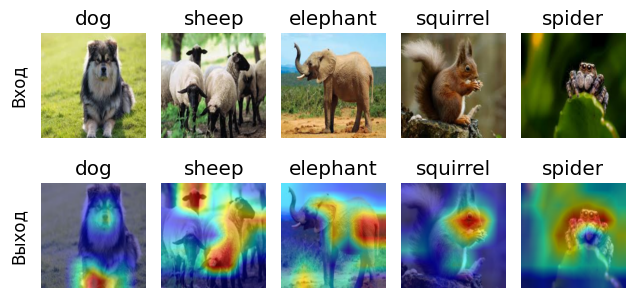
\includegraphics[width=0.8\textwidth]{images/cvgg13_out_2.png}
        \caption{\centering Результаты применения Grad-CAM к модели CVGG13 (продолжение)}
        \label{fig:cvgg13_gradcam_2}
    \end{figure}
\end{frame}

\begin{frame}{Заключение}
    В рамках работы были решены следующие задачи:
    \begin{itemize}
        \item Был изучен принцип работы сверточной нейронной сети
        \item Были изучены и реализованы архитектуры AlexNet и VGG
        \item Классификаторами была достигнута желаемая точность ($>80\%$)
        \item Проведен анализ поведения модели (Grad-CAM)
    \end{itemize}

    Таким образом, была достигнута \textbf{цель} работы.
\end{frame}

\end{document}